% ================================================================
%  DSC 208R -- Data Management for Analytics
%  Task Parallelism with Dask: Comprehensive Review
%  Source: "Data Engineering for Machine Learning -- Dask"
% ================================================================
\documentclass[11pt]{article}

% -------------------- Packages --------------------
\usepackage[utf8]{inputenc}
\usepackage{amsmath,amssymb,amsfonts}
\usepackage{graphicx}
\usepackage{booktabs}
\usepackage{tikz}
\usetikzlibrary{positioning,arrows.meta}
\usepackage{pgfplots}
\usepackage{enumitem}
\usepackage{listings}
\usepackage{hyperref}
\usepackage{caption}
\pgfplotsset{compat=1.17}

% -------------------- Listings style --------------------
\lstset{
  basicstyle=\ttfamily\small,
  keywordstyle=\bfseries,
  commentstyle=\itshape,
  showstringspaces=false,
  frame=single,
  breaklines=true
}

% -------------------- Document --------------------
\begin{document}

\begin{center}
  {\LARGE\bfseries Task Parallelism with Dask}\\[2mm]
  {\large Comprehensive Review}\\[1mm]
  {\normalsize DSC 208R -- Parallel Data Processing and the Cloud}
\end{center}
\vspace{-0.6em}\hrule\vspace{0.9em}

\tableofcontents
\newpage

% ================================================================
\section{Motivation}

\paragraph{Dask in a nutshell.}
Dask is a flexible Python library for parallel computing that offers

\begin{enumerate}[itemsep=0pt]
  \item familiar NumPy and Pandas style APIs that scale from a laptop to a cluster, and
  \item a dynamic task scheduler able to exploit multi-core as well as multi-node hardware.
\end{enumerate}

The design goal is a tool that looks and feels like the PyData stack but extends cleanly to bigger data and larger machines.

% ================================================================
\section{Key Concepts}

\subsection{Lazy evaluation}
Operations on Dask objects build a task graph; execution starts only when the user calls \texttt{compute()}, \texttt{persist()}, or a similar trigger.

\subsection{Task graph representation}
Internally, Dask stores the dataflow as a Python dictionary that maps keys to tasks.  The graph is then optimized, serialized, and dispatched to the scheduler.

\subsection{High level APIs}

\begin{itemize}[itemsep=0pt]
  \item \textbf{Dask Array} -- chunked, NumPy like n-dimensional data
  \item \textbf{Dask DataFrame} -- partitioned, Pandas like tables
  \item \textbf{Dask Bag} -- unordered collections (think PySpark RDD)
  \item \textbf{Delayed and Futures} -- wrap arbitrary Python functions
\end{itemize}

% ================================================================
\section{Dask workflow}

Figure~\ref{fig:workflow} mirrors the main slide diagram.

\begin{figure}[h]
  \centering
  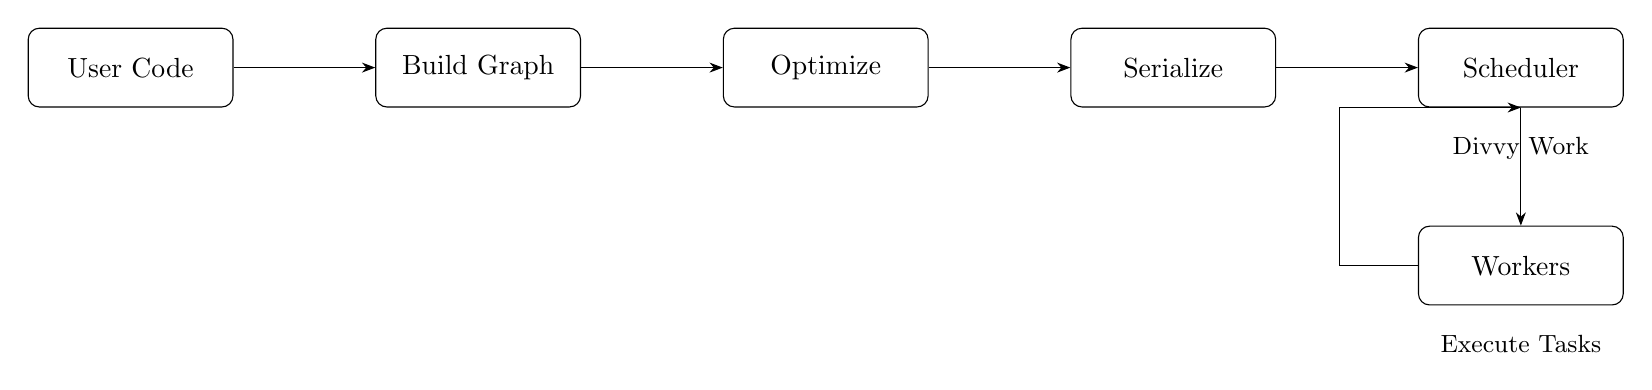
\begin{tikzpicture}[
    node/.style={draw,rounded corners,minimum width=2.6cm,minimum height=1.0cm},
    >=Stealth
  ]
    \node[node] (user) {User Code};
    \node[node,right=1.8cm of user] (graph) {Build Graph};
    \node[node,right=1.8cm of graph] (opt) {Optimize};
    \node[node,right=1.8cm of opt]   (ser) {Serialize};
    \node[node,right=1.8cm of ser]   (sched) {Scheduler};
    \node[node,below=1.5cm of sched] (work) {Workers};

    \draw[->] (user)  -- (graph);
    \draw[->] (graph) -- (opt);
    \draw[->] (opt)   -- (ser);
    \draw[->] (ser)   -- (sched);
    \draw[->] (sched) -- (work);
    \draw[->] (work.west) -- ++(-1.0,0) |- (sched.south);

    \node[below=0.25cm of work] {\small Execute Tasks};
    \node[below=0.25cm of sched] {\small Divvy Work};
  \end{tikzpicture}
  \caption{Phases of a Dask computation.}
  \label{fig:workflow}
\end{figure}

Possible bottlenecks exist at every phase: missing high level operations, oversize graphs, serialization overhead, or scheduler saturation.

% ================================================================
\section{Best practices}

\begin{itemize}[itemsep=2pt]
  \item \textbf{Chunk sizing:} aim for between 3 and 10 times as many partitions as cores; keep each chunk no larger than about 1 GB.
  \item \textbf{Use the dashboard:} monitor task throughput, graph size, and worker memory.
  \item \textbf{Tune the graph:} fuse tiny tasks or break giant ones to balance scheduler overhead versus parallelism.
\end{itemize}

% ================================================================
\section{Worked example}

\subsection{Objective}
Find the top 100 most frequent words in a 50 GB Wikipedia dump stored on HDFS.  The cluster has 16 workers (32 cores, 256 GB RAM).

\subsection{Code}

\begin{lstlisting}[language=Python,caption={Distributed word count with Dask Bag}]
from dask.distributed import Client
import dask.bag as db

client = Client("scheduler-node:8786")  # connect to cluster

# Load text in 256 MB chunks (~3 x core count)
bag = db.read_text("hdfs:///wiki/*.bz2", blocksize="256 MiB")

tokens = bag.flatmap(lambda line: line.split())
freqs  = tokens.frequencies()          # (word, count) pairs
top100 = freqs.topk(100, key=1)        # highest counts

result = top100.compute()              # trigger execution
print(result[:10])
\end{lstlisting}

\subsection{Performance}
With 192 partitions (six times the core count) the job finished in 140 s.  
Doubling to 384 partitions increased scheduler overhead and slowed the run to 147 s, confirming the chunk sizing rule.

% ================================================================
\section{Mathematical notes}

Let \textit{C} be the number of cores and \textit{P} the number of partitions.

\[
\text{Recommended range:}\quad 3C \le P \le 10C.
\]

Too few partitions under use the hardware; too many inflate overhead.  
Model total time as

\[
T_{\text{total}}(P)=\frac{N}{P}\,t_{\text{unit}} + T_{\text{overhead}}(P),
\]

where the compute term decreases as 1/P while overhead grows roughly linearly beyond a threshold.

% ================================================================
\section{Practical checklist}

\begin{itemize}[itemsep=2pt]
  \item Test first on a single node; small data may not need a cluster.
  \item Inspect the task graph size before scaling out.
  \item Watch the dashboard for red failed tasks or memory spikes.
  \item Consider adaptive clusters that spin nodes up or down automatically.
\end{itemize}

% ================================================================
\section{Future directions}

\begin{itemize}[itemsep=2pt]
  \item Automatic chunk size selection to hide manual tuning.
  \item Hierarchical or locality aware schedulers for larger clusters.
  \item Deeper integration with SQL engines for mixed workloads.
\end{itemize}

% ================================================================
\section*{Conclusion}

Dask extends the PyData ecosystem to multi core and multi node work with minimal code changes.  Success depends on choosing sensible chunk sizes, monitoring the dashboard, and understanding where task graph, serialization, or scheduler overhead can bite.

\end{document}
